\documentclass[aspectratio=169,
				xcolor=table]{beamer}
				
% Load general definitions
\usepackage[utf8]{inputenc}
%\usepackage[T1]{fontenc}
\usepackage[brazil]{babel}
\usepackage{amsmath}
\usepackage{amsfonts}
\usepackage{amssymb}
\usepackage{graphicx}
\usepackage{verbatim}
\usepackage{cancel}
\usepackage{askmaps}
\usepackage{tabularx}
\usepackage[table]{xcolor}
%\usepackage{tikz}
\usepackage{multirow}
\usepackage{mathtools}
\usepackage{color, colortbl}
\usepackage{etoolbox}
\usepackage{pbox}
\usepackage{changepage}
\usepackage{xpatch}
\usepackage{array}
\usepackage{marvosym}
\usepackage{tabu}
\usepackage{multicol}
\usepackage{listings}
\usepackage{underscore}
\usepackage{filecontents}
\usepackage[]{algorithm2e}
\usepackage{ragged2e}

\newcolumntype{P}[1]{>{\centering\arraybackslash}m{#1}}
\definecolor{Gray}{gray}{0.75}
\definecolor{Gray2}{gray}{0.85}

\definecolor{lightBlue}{HTML}{DAE8FC}
\definecolor{Blue}{RGB}{51, 51, 204}

%\useinnertheme[lily]{rounded}
\usetheme{UniEvangelica}
%\usetheme{Copenhagen}
%\usetheme{Berlin}
%\usecolortheme{dolphin}
\tolerance=1
\emergencystretch=\maxdimen
\hyphenpenalty=10000
\hbadness=10000

\setbeamertemplate{navigation symbols}{}%remove navigation symbols


\let\olditem=\item% 
\renewcommand{\item}{\olditem \justifying}%
\def\center{\trivlist \centering\item\relax}
\def\endcenter{\endtrivlist}

\setbeamertemplate{itemize/enumerate body begin}{\large}
\setbeamertemplate{itemize/enumerate subbody begin}{\large}

\setbeamertemplate{itemize item}{\raisebox{0.1ex}{$\blacktriangleright$}\hskip0.1em}
\setbeamertemplate{itemize subitem}{\raisebox{0.1ex}{$\blacktriangleright$}\hskip0.1em}

\newcommand{\greenarrow}{\textcolor{green}{\rotatebox[origin=c]{180}{\MVArrowDown}}}

\newcommand{\redarrow}{\textcolor{red}{\MVArrowDown}}

%\newcommand{\ftable}{
%	\begin{table}
%		\large
%		\centering
%		\rowcolors{1}{\ifnumless{\rownum}{2}{Blue}{lightBlue}}{}
%}

\newenvironment{eftable}{
	\begin{table}
		\large
		\centering
		\rowcolors{1}{}{Blue}
		\rowcolors{1}{\ifnumless{\rownum}{2}{Blue}{lightBlue}}{}
	}
	{
	\end{table}
}


%\setbeamertemplate{frametitle}
%{
%	%\vspace*{-2em}	
%	\insertframetitle
%
%	 %\textcolor{white}{\LARGE \insertframetitle}
%
%}

% Specific definitions
\title[]{Arquitetura e Organização de Computadores}
\subtitle[]{Memória Virtual}
\author[]{Prof. Alexandre Tannus}
\date{}

\AtBeginSection{\frame{\tableofcontents[currentsection]}}

\begin{document}

	\begin{frame}
		\titlepage
	\end{frame}

	\begin{frame}
		\tableofcontents		
	\end{frame}	
	
%	\section{Introdução}
	\begin{frame}
		\frametitle{Introdução}
		\begin{itemize}
			\item Memória virtual é a utilização de parte da memória secundária como memória principal
			\vspace{1em}
			\item Princípios semelhantes ao das memórias cache
			\begin{itemize}
				\item Localidade espacial e temporal
				\item Função de mapeamento
				\item Transparência para o programador
			\end{itemize}
			\item Caches são utilizadas para aumentar o desempenho com relação ao tempo de acesso. Memória virtual aumenta o desempenho com enfoque em capacidade de armazenamento
		\end{itemize}
		
	\end{frame}
	
	\begin{frame}
		\frametitle{Espaço de Endereçamento}
		\begin{figure}[hbtp]
		\centering
		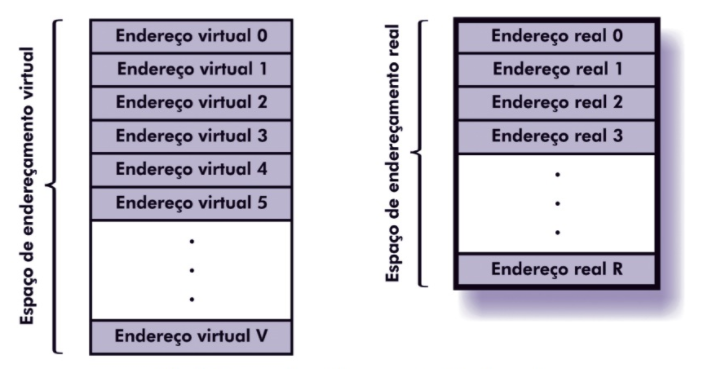
\includegraphics[height=0.75\textheight, keepaspectratio]{../figs/cap09/enderecamento.png}
		\end{figure}
		
	\end{frame}

	\begin{frame}
		\frametitle{Espaço de Endereçamento}
		\begin{figure}[hbtp]
		\centering
		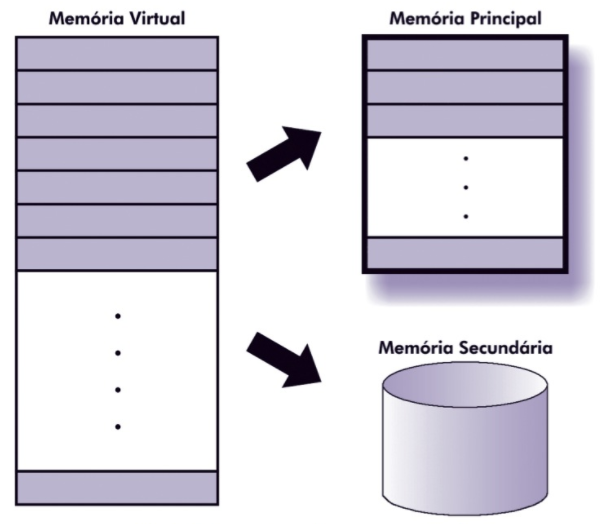
\includegraphics[height=0.75\textheight, keepaspectratio]{../figs/cap09/enderecamento2.png}
		\end{figure}
		
	\end{frame}
	
	\begin{frame}
		\frametitle{Vantagens}
		\begin{itemize}
			\item Espaço virtual pode ser muito maior que o espaço de endereçamento físico
			\vspace{1em}
			\item Suporte para coexistência de vários programas, em primeiro ou em segundo plano
			\vspace{1em}
			\item Compartilhamento de memória física ou periféricos entre processos
		\end{itemize}
	\end{frame}
	
	\begin{frame}
		\frametitle{Desvantagens}
		\begin{itemize}
			\item Possibilidade de causar lentidão no sistema por excesso de leitura/escrita no HD
		\end{itemize}
	\end{frame}
	
	\begin{frame}
		\frametitle{Tradução de endereços}
		
		\begin{itemize}
			\item Realizada via \textit{hardware} com auxílio do sistema operacional
			\vspace{1em}
			\item \textit{Hardware} responsável - \textit{Memory Management Unit} (MMU)
			\vspace{1em}
			\item Mecanismo de tradução mantém tabelas de mapeamento exclusivas para cada processo
			
		\end{itemize}
	\end{frame}
	
	\begin{frame}
		\frametitle{Tradução de endereços}
		\begin{itemize}
			\item Tabelas mapeiam blocos de dados
			\item Blocos pode ter
			\begin{itemize}
				\item Tamanho fixo - técnica de paginação
				\item Tamanho variável - técnica de segmentação
			\end{itemize}
		\end{itemize}
	\end{frame}
	
	\begin{frame}
		\frametitle{Espaço virtual x tamanho do bloco}
		
		\begin{eftable}
			\begin{tabular}{cccc}
			{\color[HTML]{FFFFFF} \begin{tabular}[c]{@{}c@{}}Espaço de \\endereçamento  virtual\end{tabular}} & 
			{\color[HTML]{FFFFFF} \begin{tabular}[c]{@{}c@{}}Tamanho do \\ Bloco\end{tabular}} & 
			{\color[HTML]{FFFFFF} \begin{tabular}[c]{@{}c@{}}Número de \\ Blocos\end{tabular}} & 
			{\color[HTML]{FFFFFF} \begin{tabular}[c]{@{}c@{}}Entradas na tabela \\ de mapeamento\end{tabular}} \\
			$2^{32}$ endereços & 
			512 endereços &                       
			$2^{23}$ & 
			$2^{23}$ \\
			$2^{32}$ endereços & 
			4k endereços &
			$2^{20}$ & 
			$2^{20}$ \\
			$2^{64}$ endereços  & 
			4k endereços &  
			$2^{52}$ & 
			$2^{52}$ \\
			$2^{64}$ endereços & 
			64k endereços &
			$2^{48}$ & 
			$2^{48}$                                                                                      
			\end{tabular}
		\end{eftable}
	\end{frame}
	
	\begin{frame}
		\frametitle{Política de demanda de páginas}
		
		\begin{itemize}
			\item Determina quando uma página deve ser carregada
			\vspace{1em}
			\item Dois tipos
			\begin{itemize}
				\item Por demanda
				\item Antecipada
			\end{itemize}
		\end{itemize}
	\end{frame}
	
	\begin{frame}
		\frametitle{Política de alocação de páginas}
		
		\begin{itemize}
			\item Determina quantos \textit{frames} cada processo pode manter na memória principal
			\vspace{1em}
			\item Dois tipos
			\begin{itemize}
				\item Fixa
				\item Variável
			\end{itemize}
			
		\end{itemize}
	\end{frame}
	
	\begin{frame}
		\frametitle{Política de substituição de páginas}
		\begin{itemize}
			\item Define qual página será retirada da memória quando outra precisar ser alocada
			\vspace{1em}
			\item Deve ser considerada a ocorrência de modificações na página
			\vspace{1em}
			\item Local ou global
			
		\end{itemize}
		\begin{figure}[hbtp]
		\centering
		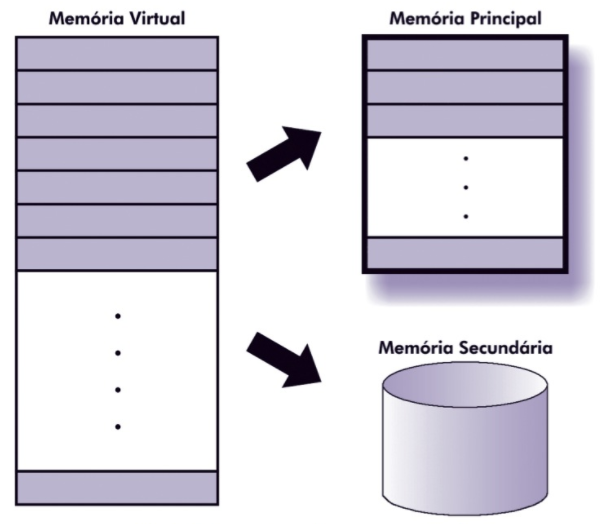
\includegraphics[height=0.4\textheight, keepaspectratio]{../figs/cap09/enderecamento2.png}
		\end{figure}
	\end{frame}
	
	\begin{frame}
		\frametitle{Algoritmos de substituição de páginas}
		
		\begin{itemize}
			\item Ótimo 
			\item Aleatório
			\item FIFO (\textit{First In First Out})
			\item LFU (\textit{Least Frequently Used})
			\item LRU (\textit{Least-Recently-Used})
			\item NRU (\textit{Not-Recently-Used})
			\item FIFO com \textit{buffer} de páginas
			\item FIFO circular


		\end{itemize}
	\end{frame}

\end{document}